\chapter{ChatScript: Grundlagen}
\label{sec:ChatScript: Grundlagen}

Bei ChatScript handelt es sich um ein Framework, der es Entwicklern erlaubt, regelbasierte Chatbots zu entwickeln. Es handelt sich hierbei um "Natural Language tool" mit eigenem Interpreter, welcher Code in C++ übersezt. 


\section{Regeln}
\label{sec:ChatScript: Regeln}

Regeln sind ein elementarer Bestandteil in ChatScript. In diesen Regeln wird unter Anderem Nutzereingaben analysiert, Antworten des Bots festgelegt, Datenbankabfragen ausgeführt und der Gesprächsablauf gesteuert.  

In Augusta finden sich Regeln in verschiedenen Formen wieder. Diese sind: 

\begin{itemize}
\item t: für Ausgaben des Chatbots, ohne folgende Antwort 
\item u: für Ausgaben in Form von Fragen, das beduetet, dass auf Regeln mit u: eine Antwort des Nutzers folgen muss 
\item a:, b:, c: etc. für Antworten des Nutzers. Auf diese Regeln können Pattern-Matching-Ansätze angewandt werden, um Teile der Eingabe ggf. zu extrahieren.
\end{itemize}

Topics haben, auch wenn optional, meist einen Bezeichner, eine Bedingung zur Ausführung und es lassen sich dabei Variablen zuweisen. Ein abstraktes Beispiel:

\begin{lstlisting}[caption={Syntax für Regeln}]
t: BEZEICHNER (KONDITION) \$meineVariable=Wert Ausgabe des Bots
\end{lstlisting}

Im folgenden einige Beispiele für Regeln:

\begin{lstlisting}[caption={Beispiel für t:}]
t:  ( %input<%userfirstline )
    ^keep()
    [Hallo] [Hi] [Guten Tag], ich bin Augusta und kann dich beraten, wenn du etwas aus dem Online-Shop suchst. ^reuse( GREET )
\end{lstlisting}

In dieser Regel wird der Nutzer begrüßt und im Folgenden der Gesprächsverlauf zur Regel GREET weitergeleitet.

\begin{lstlisting}[caption={Beispiel für Gesprächsablauf mit Antworten u:, a: und b:}]
 u: INTRO (\$enter211) [Das ist gut] [Das ist toll] [Das freut mich], [dabei kann ich dir helfen] [ich kann dir dabei helfen, etwas zu finden] [ich kann dich beraten]. Also dann, wollen wir loslegen DEBUG?

		a: ( ~positiv ) \$introyes = 1a
	# DATENBANK
	    if (^dbinit(dbname = postgres port = 5432 user = postgres password = 1234))
	        {[Lass uns anfangen] [Super, auf geht's]!  ^reuse( FIRSTQ )
	    } else {dbinit failed - \$$db_error  ^reuse( FIRSTQ ) }
	a: ( ~negativ ) Tut mir Leid, ich kann eigentlich nur beraten. Bist du dir sicher, dass du nichts aus dem Shop möchtest?
		b: ( ~negativ )  \$introyes = 1a if (^dbinit(dbname = postgres port = 5432 user = postgres password = 1234 )) {Schön zu hören. ^reuse( FIRSTQ )}
                                      else {dbinit failed - \$$db_error ^reuse(FIRSTQ)}
	    b: ( ~positiv ) \$enterEnd2 = 1b Das ist schade. ^reuse( ~ende.ASKIFHAPPY )
\end{lstlisting}

In diesem Abschnitt fragt der Bot mit zufällig ausgewählter Frage, ob der Kunde etwas kaufen möchte. Falls die Eingabe des Kunden ein Wort aus dem Konzept ~positiv enthält, wird entsprechend die Datenbank geladen und in die Regel FIRSTQ im selben Topic aktiviert. Falls die Eingabe ein Wort aus dem Konzept ~negativ enthält, so wird gefragt, ob man nicht wirklich was sucht. Je nach Antwort darauf wird eine entsprechende Regel, d.h. eines der beiden b: Regeln ausgeführt. 


\section{Topics}
\label{sec:ChatScript: Topics}

Die Quelldateien in einem ChatScript-Programm werden auch als "`Topics"' bezeichnet und haben die Dateiendung .top. Topics können als Zusammenfassung mehrerer Regeln betrachtet werden. Es bietet sich an, Topics als Module eines Chatbots zu handhaben. So wird z.B. in diesem Projekt "`Augusta"' die Datenbankabfrage als eignenes Topic gehandhabt.
Topics beginnen immer mit einer Tilde ("`~"') als Präfix gefolgt vom Topicnamen, meist als erste Zeile in einer .top-Datei oder vor dem Auflisten von Regeln:

\begin{lstlisting}[caption={Topicbezeichner in dbsearch.top}]
topic: ~dbsearch  [] (\$gosearch)
\end{lstlisting}


\section{Konzepte}
\label{sec:ChatScript: Konzepte}

Syntaktisch werden Konzepte wie Topics gehandhabt, das heißt, dass Konzepte mit ~Konzeptname referenziert werden. Ein Konzept kann als eine Menge von Synonymen verstanden werden, ähnlich zu Einträgen in einem Thesaurus. Obwohl es sich hier um Mengen handelt, stehen diese aus syntaktischer Sicht in Klammern () oder []. Ein Beispiel anhand des Konzepts "`~ciao"':

\begin{lstlisting}[caption={Konzept 'ciao' aus konzepte.top}]
concept: ~ciao [ciao tschüss "good bye" bye "daje" "eddi un merci" "äddi a merci"]
\end{lstlisting}

Anzumerken ist, dass Ausdrücke aus mehreren Wörtern, sogenannte "`multiword expressions"', in Anführungszeichen stehen müssen, da die einzelnen Bestandteile dieser sonst als einzelne Elemente betrachtet werden.


In "`Augusta"' sind Konzepte besonders wichtig, da es sich anbietet, das Pattern-Matching von Konzepten abhängig zu machen. So wird mit Hilfe von Konzepten das Arbeiten mit der PostgreSQL-Schnittstelle gewährleistet: Für jeden möglichen Eintrag pro Spalte in der PostgreSQL-Datenbank existiert ein Konzept. Als Beispiel alle Einträge für die Spalte "`Anwendungszweck"' (zur Datenbank s. \ref{sec:DB}):  

\begin{lstlisting}[caption={Konzept 'anwendungszweck' aus konzepte.top}]
concept: ~anwendungszweck [Unterhaltung Schreibwaren EssenTrinken Essentrinken Alltag Accessoire]
\end{lstlisting}

Der Nutzer beschreibt beispielsweise in einem Satz, welchen Anwendungszweck das gesuchte Produkt erfüllen soll. Wird ein Wort aus dem Konzept gefunden, so wird dieses als solches erkannt, \textcolor[rgb]{1,0.41,0.13}{sofern vom Skript vorgesehen.} Damit wird sichergestellt, dass in den Queries nur Eigenschaften vorkommen, die in Datenbankeinträgen existieren. Sollte der Anwender nach Eigenschaften suchen, die nicht existieren, so werden diese ignoriert (zum Pattern-Matching s. \ref{sec:ChatScript: Pattern-Matching} und zur Query s. \ref{sec:SQL}). 

\textcolor[rgb]{1,0.41,0.13}{Des Weiteren erlaubt es ChatScript, mehrere verschiedene Konzepte in einem Konzept zu vereinen. Ein solches Konzept ist als Vereinigung mehrerer Konzepte zu verstehen: Diese Sätze sind doppeltgemoppelt}

\begin{lstlisting}[caption={Konzept 'positivkaufen' aus konzepte.top}]
concept: ~positivkaufen [ ~yes ~zustimmung ~kaufen]
\end{lstlisting}

'~positivkaufen' enthält somit alle Wörter, die in ~yes, ~zustimmung und ~kaufen vorkommen. 

\section{ChatScript: Variablen}
\label{sec:ChatScript: Variablen}
Variablen in Augusta kommen größtenteils in der Form \$variablenname vor. \$ vor dem Identifier bedeutet, dass diese Variable permanent \textcolor[rgb]{1,0.41,0.13}{global?} ist und über die Regel hinaus existiert. Variablen werden für gewöhnlich im Kopf einer Regel instanziiert. Bei den zugewiesenen Werten kann es sich um eine Konstante handeln oder Werte, die mit Hilfe von Pattern-Matching gefunden und aus der Antwort des Benutzers extrahiert werden. Im folgenden Beispiel wird das erste Wort der Nutzereingabe, welches sich im Konzept ~geschenkidee befindet in der Variable \$geschenkidee gespeichert. 

\begin{lstlisting}[caption={Zuweisung des Wertes einer Variable }]
a: ( _~geschenkidee ) \$anwendungszweck = ^"'nichts'" \$geschenkidee = ^"''_0'"}
\end{lstlisting}

Bereits instanziierte Variablen lassen sich einsehen mit dem Befehl \lstinline|^walkvariables|(\^outputmacro) einsehen. 

Da das Zurücksetzen von Variablen nicht trivial ist, lassen sich diese mit dem Befehl \lstinline|^reset( VARIABLES )| zurücksetzen. Dieser Befehl setzt alle Variablen auf globaler Ebene zurück. Wenn man verhindern möchte, dass eine Variable zurückgesetzt wird, empfiehlt es sich diese als temporäre Variable zwischenzuspiechern, wie folgt:


\begin{lstlisting}[caption={Zwischenspeichern einer Variable}]
	\$_cs_bottmp = \$cs_bot
    ^reset( VARIABLES )
    #....
	\$cs_bot = \$_cs_bottmp 
\end{lstlisting}

Dieser Schritt findet in ende.top statt. Dies ist nötig, um zu gewährleisten, dass sowohl Informationen wie der Name des Kunden als auch die Insatz des Bots nicht verloren gehen, wenn eine weitere Empfehlung im selben Gespräch erfolgen soll. 


\section{Variablen als Bedingungen zur Steuerung von Programmablauf}
\label{sec:ChatScript: Variablen als Bedingungen zur Steuerung von Programmablauf}

Nativ wählt ChatScript Regeln in einem Topic zufällig aus, um durch themenbezogene zufällige Antworten natürlich zu wirken. Da Augusta, ein Chatbot zur Kaufberatung, jedoch eine lineare Konversation gewährleisten muss, wird in fast allen Regeln mit Bedingungen gearbeitet. Ein Beispiel: 

\begin{lstlisting}[caption={Regelkopf von FIRSTQ in kaufabsicht.top}]
u: FIRSTQ (\$introyes) Wir können nach etwas zum ... 
\end{lstlisting}

Die Regel FIRSTQ darf nur aktiviert werden, sofern die Variable \$introyes existiert. 

Ähnlich lässt es sich auch verhindern, dass der Bot in eine Regel übergeht, indem man Variablen als Bedingungen stellt, die in keiner Regel instanziiert werden:

\begin{lstlisting}[caption={Regelkopf von STARTKAUF in kaufabsicht.top}]
t: STARTKAUF (\$enter999) ^reuse( INTRO)
\end{lstlisting}

Die Regel Startkauf ist gewöhnlich nicht betretbar für den Bot, da \$enter999 als Variable nie instanziiert wird. Selbiges gilt für alle Regeln, dessen Bedingung die Existenz einer Variable mit '\$enter...' erfordert. Diese Bedingungen dienen dazu, um ein zufälliges Springen des Bots zu verhindern. \textcolor[rgb]{1,0.41,0.13}{Stattdessen} muss manuell von einer Regel auf diese weitergeleitet werden, was mit Hilfe von Befehlen zur Steuerung des Programmablaufs erfolgt. 

Alternativ, jedoch nicht so häufig, ist die Bedingung, dass ein Wort eines Konzepts zu erwähnen ist, damit eine Regel betreten wird:

\begin{lstlisting}[caption={Regelkopf einer Regel in kaufabsicht.top}]
b: (~willGeschenk) \$anwendungszweck = ^"'nichts'" Du möchtest etwas verschenken. Ich kann dir folgende Kategorien anbieten:
\end{lstlisting}

Diese Regel, sofern erreichbar, erfordert von der Nutzereingabe, dass ein Wort aus dem Konzept '~willGeschenk' erwähnt wird. Ist dies nicht der Fall, so wird auch nicht in diese Regel übergegangen.


\section{Befehle zur Steuerung von Programmablauf}
\label{sec:ChatScript: Befehle zur Steuerung von Programmablauf}

In Augusta wurden zwei Methoden genutzt, um den Gesprächverlauf zu lenken. Dabei handelt es sich zum einen um \lstinline|^gambit(~topic)| und zum anderen um \lstinline|^reuse(~topic.rule)|. Im Laufe des Projekts hat sich \lstinline|^reuse(~topic.rule)| als praktischer herausgestellt, da man direkt in Regeln desselben Topics als auch in Regeln anderer Topics springen kann. Des Weiteren ignoriert \lstinline|^reuse| die Bedingungen der Zielregel, sodass Regeln betreten werden, unabhängig davon, ob ein Wort des geforderten Konzepts oder die geforderte Variable existiert. Sofern sich eine Regel im selben Topic befindet, muss in \lstinline|^reuse| nur die Zielregel angegeben werden:

\begin{lstlisting}[caption={Regel STARTKAUF in kaufabsicht.top}]
t: STARTKAUF (\$enter999) ^reuse( INTRO)
\end{lstlisting}

Wird die Regel 'STARTKAUF' betreten, so wird am Ende der Ausführung in die Regel 'INTRO' desselben Topics übergegangen. 

\begin{lstlisting}[caption={Regel in keyexonesentence.top}]
a: (~positiv) \$gosearch = 1c Alles klar! Ich suche mal im Shop. d3 ^reuse( ~dbsearch.WELCOME )
\end{lstlisting}

Sofern ein Wort aus dem Konzept '~positiv' aus der Nutzereingabe erkannt und ist diese Regel betretbar, so wird diese Regel ausgeführt und anschließend die Regel 'WELCOME' in dbsearch.top, einem anderen Topic, betreten.

Im Verlauf der Entwicklung wurde \lstinline|^gambit| mit \lstinline|^reuse| ersetzt, da \lstinline|^reuse| eine präzisere Steuerung des Programmablaufs erlaubt. Während \lstinline|^gambit| lediglich in eine anderes Topic springt und dieses von der ersten betretbaren Regel an ausführt, lässt sich durch \lstinline|^reuse| festlegen, welche Regel zu betreten ist, ohne auf die Bedingung der Zielregel achten zu müssen.  


\section{Pattern-Matching}
\label{sec:ChatScript: Pattern-Matching}

\textcolor[rgb]{1,0.41,0.13}{Schreiben über:}

ChatScripts Interpreter bietet einen hauseigenen Pattern-Matcher zum Vergleichen von Nutzereingaben. Diese Ansätze eignen sich an erster Stelle dazu, Bedingungen für Regeln zu schreiben. Die einfachste Form, um eine Nutzereingabe abzugleichen, ist, zu überprüfen, ob Nutzereingaben ein aus Konzepten bekanntes Token enthalten. Die folgende Regel überprüft, ob die Nutzereingabe ein Wort aus dem Konzept '~positiv' enthält. Ist dies der Fall und ist die Regel erreichbar, so wird die folgende Regel ausgeführt:

\begin{lstlisting}[caption={Regel in kaufabsicht.top}]
c: ( ~positiv ) \$enterEnd2 = 1b Das ist schade. ^reuse( ~ende.ASKIFHAPPY )
\end{lstlisting}

Es besteht des Weiteren die Möglichkeit, eine Nutzereingabe auf mehrere Konzepte zu überprüfen: 

\begin{lstlisting}[caption={Regel in kaufabsicht.top}]
b: ( [~no ~nicht] ) \$enterEnd2 = 1b In Ordnung. ^reuse( ~ende.ASKIFHAPPY )
\end{lstlisting}

Außerdem stellt ChatScript Mittel bereit, um Aussagen über die Reihenfolge von Wörtern in einer Nutzereingabe zu treffen. Im Folgenden wird überprüft, ob das Wort 'nicht' in derselben Nutzeringabe wie ein Wort aus dem Konzept sagen vorkommt. Dabei wird nicht eingeschränkt, an welchem Index die Wörter in der Nutzereingabe vorkommen, sodass Nutzereingaben wie 'Das will ich nicht verraten' oder 'Nicht das will ich verraten' von dieser Bedingung akzeptiert werden. 

\begin{lstlisting}[caption={Regel KEINE\_VORSTELLUNG in introductions.top}]
a: KEINE_VORSTELLUNG (<<[sagen] nicht>>) [Das verstehe ich] [Das kann ich nachvollziehen]. ^reuse(~kaufabsicht.STARTKAUF)
\end{lstlisting}

Interessanter wird es, wenn Wörter aus Nutzereingaben extrahiert werden müssen. Für diesen Zweck bietet ChatScript Wildcards der Form *n. Diese erlauben es, Token an einer bestimmten Stelle zu extrahieren und ggf. in einer Variable zu speichern. 

\begin{lstlisting}[caption={Regel in introductions.top}]
a: VORSTELLUNG ([heiße bin ist lautet] _*1 >)
	    if (\$cs_token == \$stdtoken)
           {
           \$cs_token = #DO_INTERJECTION_SPLITTING |
                       #DO_SUBSTITUTE_SYSTEM | #DO_NUMBER_MERGE |
                       #DO_PARSE
           retry(SENTENCE)
           }
        \$kunde =  pos(noun '_0 proper)
\end{lstlisting}

Im Grunde wird hier das erste Wort nach 'heiße', 'bin', 'lautet' oder 'ist' genommen und nach Verarbeitung in der Variable \$kunde gespeichert. 

Wildcards spielen in Augusta eine zentrale Rolle, wenn es darum geht, Kundenwünsche zu verarbeiten. In keyexonesentence.top finden sich verschiedene Muster zum Verständnis von Kundenwünschen. Dabei wird drauf geachtet, dass Wörter erwähnt werden, die in den Konzepten entsprechend vorkommen, sodass eine Query anhand der gegebenen Wörtern möglich ist: 

\begin{lstlisting}[caption={Muster 1 in keyexonesentence.top}]
    a: ( !!~positiveinteger * _~thingsandart {in} _~ausfuehrung * {_~positiveinteger} *  )
    # a: ( < {Ich} {möchten wollen suchen} {ein eine einen} _~thingsandart * {in}  _~ausfuehrung *  {für Preis Wert} * {_~positiveinteger} * )
        # Test, ob _0 Name oder Art ist
        if (pattern _0~things) {\$things = ^"''_0'" zusammenfassung = ^join(\$zusammenfassung ^" Das Produkt heißt \$things.")
        } else {\$art = ^"''_0'"  \$zusammenfassung = ^join(\$zusammenfassung ^" Dein Produkt fällt unter den Obergriff \$art.")}
        \$ausfuehrung = ^"''_1'"
        # Optionaler Preis
        if ( _2 AND ^isnumber(_2) ) {\$preis = ^"''_2'" \$zusammenfassung = ^join(\$zusammenfassung ^" Es ist in \$ausfuehrung und maximal soll es \$preis Euro kosten.")
        } else {\$zusammenfassung = ^join(\$zusammenfassung ^" Es soll in \$ausfuehrung sein und eine preisliche Obergrenze hast du nicht angegeben.")}
        1. MUSTER
        ^reuse( SUMMARY )
\end{lstlisting}
        
In diesem Pattern wird anfangs gesagt, dass eine positive Zahl nicht zu Beginn auftauchen darf. Es dürfen beliebig viele Token kommen, bis das erste Token aus dem Konzept '~thingsandart' erwähnt wird, optionaler Weise gefolgt von einem 'in' und einem Begriff aus dem Konzept '~ausfuehrung'. Darauf dürfen dann beliebig viele weitere Token folgen. Es ist freigestellt, ob darauf noch eine positive Zahl zur angabe von Preis kommt. Dabei stehen \_0, \_1, \_2 etc. für das erste, zweite, dritte erkannte Wort auf Konzepten. Im Folgenden wird in einer if-Abfrage ermittelt, ob es sich bei dem ersten Wort um ein Token aus dem Konzept '~things' oder '~art' handelt und entsprechend eine Rückmeldung gegeben. 
Insgesamt 11 verschiedene Pattern dieser Art kommen in keyonesentence vor, aufgrund der Tatsache, dass der Nutzer frei angeben kann, wann er Angaben zu Name des Gegenstands Art, Ausführung oder Preis macht. 


\section{Zufällige Ausgabe}
\label{sec:ChatScript: Zufällige Ausgabe}

ChatScript erlaubt es, dass an einer Stelle mehrere Ausgaben durch den Bot möglich sind. Mögliche Ausgaben werden mit Hilfe von [] unterschieden:

u: INTRO (\$enter211) [Das ist gut] [Das ist toll] [Das freut mich], [dabei kann ich dir helfen] [ich kann dir dabei helfen, etwas zu finden] [ich kann dich beraten]. Also dann, wollen wir loslegen DEBUG?

\begin{lstlisting}[caption={Regel in keyexonesentence.top}]
u: INTRO (\$enter211) [Das ist gut] [Das ist toll] [Das freut mich], [dabei kann ich dir helfen] [ich kann dir dabei helfen, etwas zu finden] [ich kann dich beraten]. Also dann, wollen wir loslegen DEBUG?
\end{lstlisting}

Hier wählt der Bot zufällig aus, ob 'Das ist gut', 'Das ist toll' etc. ausgegeben wird gefolgt von 'Also dann ...'.



\chapter{Augusta: Programmlogik}
\label{sec:Augusta: Programmlogik}

Da ChatBot Augusta im Grunde ein Deterministischer Automat ist, bietet es sich an, den Programmablauf als Automaten zu beschreiben. Im Folgenden wird der Programmablauf als Automat auf .top-Dateien aufgeteilt dargestellt. Dabei beschreiben Zustände die jeweiligen Regeln in Augusta. 
Folgendes gilt:

\begin{enumerate}
\item{A ist die erste Regel die aufgerufen wird in introductions.top} % Klammern geändert: Jetzt {} statt [] da das sonst am linken Rand abgeschnitten ist
\item{A.2 ist introductions.vorstellung}
\item{A.3 ist introductions.KEINE\_VORSTELLUNG}
\item{B.1 ist kaufabsicht.Startkauf}
\end{enumerate}

Für introductions gilt: Anfangs grüßt der Bot den Nutzer, geht in Regel 'GREET' über und fragt den Nutzer ob dieser seinen Namen verraten will. Je nachdem, ob aus der Nutzereingabe ein Name erkannt wird (siehe Abschnitt: Pattern-Matching) wird in die Regel 'VORSTELLUNG' bzw. 'KEINE\_VORSTELLUNG' übergegangen. Daraufhin wird die Regel 'STARTKAUF' des Topics kaufabsicht betreten. 

\begin{center}
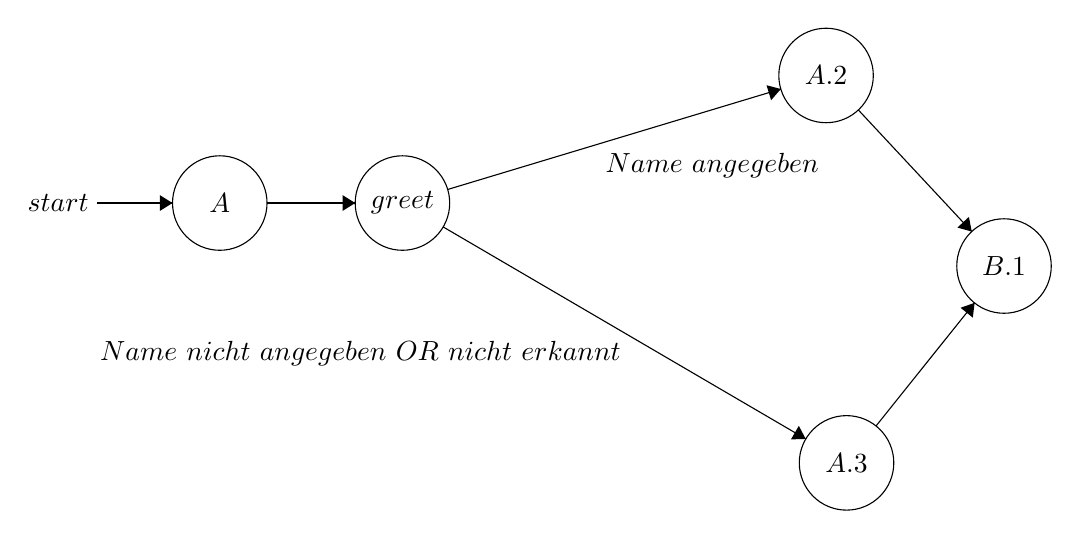
\begin{tikzpicture}[scale=0.2]
\tikzstyle{every node}+=[inner sep=0pt]
\draw [black] (11.5,-26.9) circle (3);
\draw (11.5,-26.9) node {$A$};
\draw [black] (50,-18.8) circle (3);
\draw (50,-18.8) node {$A.2$};
\draw [black] (51.3,-43.4) circle (3);
\draw (51.3,-43.4) node {$A.3$};
\draw [black] (23.1,-26.9) circle (3);
\draw (23.1,-26.9) node {$greet$};
\draw [black] (61.3,-30.9) circle (3);
\draw (61.3,-30.9) node {$B.1$};
\draw [black] (3.7,-26.9) -- (8.5,-26.9);
\draw (3.2,-26.9) node [left] {$start$};
\fill [black] (8.5,-26.9) -- (7.7,-26.4) -- (7.7,-27.4);
\draw [black] (14.5,-26.9) -- (20.1,-26.9);
\fill [black] (20.1,-26.9) -- (19.3,-26.4) -- (19.3,-27.4);
\draw [black] (25.97,-26.04) -- (47.13,-19.66);
\fill [black] (47.13,-19.66) -- (46.22,-19.42) -- (46.51,-20.37);
\draw (42.77,-23.71) node [below] {$Name\mbox{ }angegeben$};
\draw [black] (25.69,-28.42) -- (48.71,-41.88);
\fill [black] (48.71,-41.88) -- (48.27,-41.05) -- (47.77,-41.91);
\draw (20.43,-35.67) node [below] {$Name\mbox{ }nicht\mbox{ }angegeben\mbox{ }OR\mbox{ }nicht\mbox{ }erkannt$};
\draw [black] (53.17,-41.06) -- (59.43,-33.24);
\fill [black] (59.43,-33.24) -- (58.54,-33.55) -- (59.32,-34.18);
\draw [black] (52.05,-20.99) -- (59.25,-28.71);
\fill [black] (59.25,-28.71) -- (59.07,-27.78) -- (58.34,-28.46);
\end{tikzpicture}
\end{center}



Folgendes gilt:

\begin{enumerate}
\item{B.1 ist startkauf}
\item{B.2 ist die Nachfrage, ob ein Kaufwunsch besteht}
\item{B.3 ist die Regel nach Angabe, dass man ein Geschenk bzw. etwas zu einer Anwendung will}
\item{X.A ist ENDE.ASKIFHAPPY}
\item{C.1 ist keyexprodukteigenschaften.startprodukteigenschaften bzw. keyexonesentence.startkauf}
\item{Ansonsten sind die Zustände nach ihren Regeln benannt}
\end{enumerate}

Von der Regel 'STARTKAUF' geht der Bot über in INTRO und fragt, ob ein Kaufwunsch besteht. Dies wird so lange erfragt, bis der Bot die Antwort des Nutzers verstanden hat. 
Ist dies nicht der Fall, erfolgt erneute Nachfrage. Bestätigt der Nutzer, dass kein Kaufwunsch besteht, so wird dieser zu Regel 'ASKIFHAPPY' in Topic 'ENDE' weitergeleitet. Besteht doch ein Kaufwunsch, so wird in die Regel 'FIRSTQ' weitergeleitet. Sollten Probleme mit der Initialisierung der Datenbank auftreten, so wird dieser Zustand so lange wiederholt, bis die Datenbank aktiviert werden kann. 
Daraufhin wird der Nutzer gefragt, ob dieser etwas zum Schenken oder nach einem Zweck sucht. Nennt der Nutzer nur, dass er ein Geschenk bzw. etwas für einen Zweck sucht, so wird ihm mit Hilfe einer Datenbankquery vorgeschlagen, welche Geschenkzwecke bzw. Anwendungszwecke zur Verfügung stehen. Der Nutzer muss einen der aufgelisteten Geschenkideen/Anwendungszwecke nennen, welche als Variable abgespeichert werden. Nennt der Nutzer stattdessen direkt, was für eine Geschenkidee oder Anwendungszweck er möchte und ist dies auch bekannt, dann muss die Absicht nicht weiter konkretisiert werden und wird abgespeichert. 
Im folgenden betritt der Bot die Regel keyexprodukteigenschaften.startprodukteigenschaften bzw. keyexonesentence.startkauf, abhängig vom vorliegenden Ansatz (beide Ansätze im Projekt enthalten). 

\begin{center}
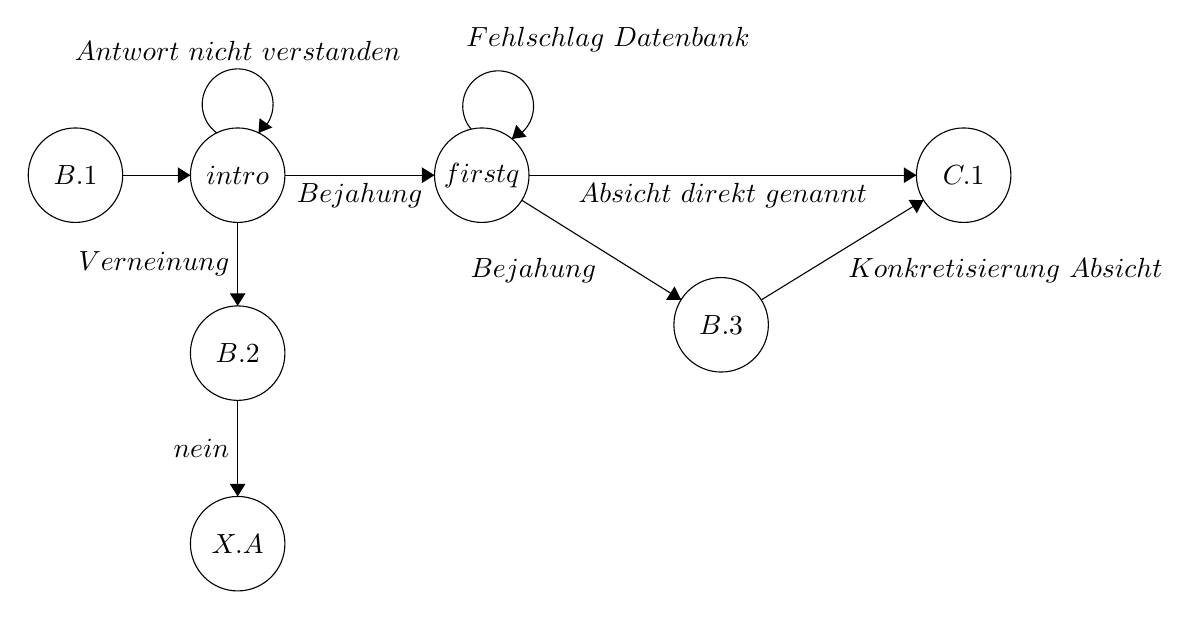
\begin{tikzpicture}[scale=0.2]
\tikzstyle{every node}+=[inner sep=0pt]
\draw [black] (4.7,-30) circle (3);
\draw (4.7,-30) node {$B.1$};
\draw [black] (15,-30) circle (3);
\draw (15,-30) node {$intro$};
\draw [black] (15,-41.3) circle (3);
\draw (15,-41.3) node {$B.2$};
\draw [black] (15,-53.4) circle (3);
\draw (15,-53.4) node {$X.A$};
\draw [black] (30.5,-30) circle (3);
\draw (30.5,-30) node {$firstq$};
\draw [black] (45.7,-39.5) circle (3);
\draw (45.7,-39.5) node {$B.3$};
\draw [black] (61.1,-30) circle (3);
\draw (61.1,-30) node {$C.1$};
\draw [black] (7.7,-30) -- (12,-30);
\fill [black] (12,-30) -- (11.2,-29.5) -- (11.2,-30.5);
\draw [black] (15,-33) -- (15,-38.3);
\fill [black] (15,-38.3) -- (15.5,-37.5) -- (14.5,-37.5);
\draw (14.5,-35.65) node [left] {$Verneinung$};
\draw [black] (15,-44.3) -- (15,-50.4);
\fill [black] (15,-50.4) -- (15.5,-49.6) -- (14.5,-49.6);
\draw (14.5,-47.35) node [left] {$nein$};
\draw [black] (18,-30) -- (27.5,-30);
\fill [black] (27.5,-30) -- (26.7,-29.5) -- (26.7,-30.5);
\draw (22.75,-30.5) node [below] {$Bejahung$};
\draw [black] (13.677,-27.32) arc (234:-54:2.25);
\draw (15,-22.75) node [above] {$Antwort\mbox{ }nicht\mbox{ }verstanden$};
\fill [black] (16.32,-27.32) -- (17.2,-26.97) -- (16.39,-26.38);
\draw [black] (33.5,-30) -- (58.1,-30);
\fill [black] (58.1,-30) -- (57.3,-29.5) -- (57.3,-30.5);
\draw (45.8,-30.5) node [below] {$Absicht\mbox{ }direkt\mbox{ }genannt$};
\draw [black] (48.25,-37.92) -- (58.55,-31.58);
\fill [black] (58.55,-31.58) -- (57.6,-31.57) -- (58.13,-32.42);
\draw (63.75,-35.26) node [below] {$Konkretisierung\mbox{ }Absicht$};
\draw [black] (33.04,-31.59) -- (43.16,-37.91);
\fill [black] (43.16,-37.91) -- (42.74,-37.06) -- (42.21,-37.91);
\draw (33.77,-35.25) node [below] {$Bejahung$};
\draw [black] (29.834,-27.087) arc (220.60377:-67.39623:2.25);
\draw (38.52,-22.23) node [above] {$Fehlschlag\mbox{ }Datenbank$};
\fill [black] (32.41,-27.7) -- (33.34,-27.56) -- (32.69,-26.8);
\end{tikzpicture}
\end{center}


Folgendes gilt:

\begin{enumerate}
\item{C.1 ist STARTPRODUKTEIGENSCHAFTEN}
\item{C.2a ist ASKNAME}
\item{C.2b ist KIND}
\item{C.3 ist DESIGN}
\item{C.4 ist PRICE }
\item{C.5 ist Summary }
\item{D.1 ist ~dbsearch.welcome }
\end{enumerate}


Wird der Ansatz Keyexprodukteigenschaften gewählt, so erfolgt ein Erfragen für die einzelnen Eigenschaften. In der Regel gilt: Werden in den Eingaben Stichworte erkannt, die als Eigenschaften in der Datenbank bekannt sind, so werden diese in Variablen gespeichert (siehe \ref{ChatScript: PatternMatching}) Zunächst wird gefragt, ob der Nutzer sein gewünschtes Produkt beim Produktnamen kennt. Ist dies nicht der Fall oder wird die Eingabe nicht als solches identifiziert, wird gefragt, ob der Nutzer weiß, von welcher 'Art', z.B. Kleidung, Verzehrmittel seine Idee ist. Erfolgt eine Eingabe, die im Konzept ~art bekannt ist, so wird in der entsprechenden Variable 'art' dieser Wert gespeichert. 
Daraufhin wird gefragt, ob man was zur Ausführung, z.B. Farbe oder Sprache, sagen kann. Wird eine bekannte Ausführung erkannt, so wird diese gespeichert, ansonsten wird die Eingabe ignoriert. 
Im Anschluss wird gefragt, welchen Preis man maximal Zahlen will. Hierbei muss eine positive Integerzahl angegeben werden als Preislimit. 
In 'SUMMARY' wird zusammengefasst, was der Bot erkennen konnte und fragt den Nutzer, ob dies dem Nutzerwunsch entspricht. Ist dies der Fall, so betritt der Bot die Regel 'Welcome' in dbsearch, ansonsten fängt man bei 'startprodukteigenschaften' von Vorne an. 



\begin{center}
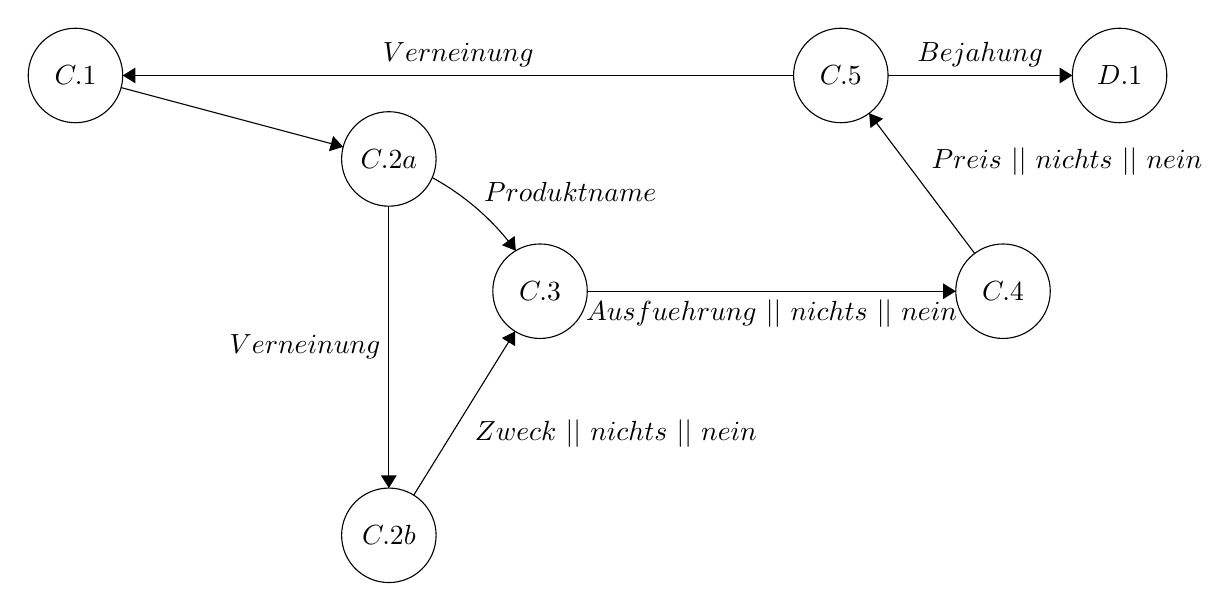
\begin{tikzpicture}[scale=0.2]
\tikzstyle{every node}+=[inner sep=0pt]
\draw [black] (8.2,-16.1) circle (3);
\draw (8.2,-16.1) node {$C.1$};
\draw [black] (28.1,-21.4) circle (3);
\draw (28.1,-21.4) node {$C.2a$};
\draw [black] (28.1,-45.3) circle (3);
\draw (28.1,-45.3) node {$C.2b$};
\draw [black] (37.7,-29.8) circle (3);
\draw (37.7,-29.8) node {$C.3$};
\draw [black] (67.1,-29.8) circle (3);
\draw (67.1,-29.8) node {$C.4$};
\draw [black] (56.8,-16.1) circle (3);
\draw (56.8,-16.1) node {$C.5$};
\draw [black] (74.5,-16.1) circle (3);
\draw (74.5,-16.1) node {$D.1$};
\draw [black] (11.1,-16.87) -- (25.2,-20.63);
\fill [black] (25.2,-20.63) -- (24.56,-19.94) -- (24.3,-20.91);
\draw [black] (30.852,-22.584) arc (61.41227:36.21588:16.173);
\fill [black] (36.16,-27.23) -- (36.09,-26.29) -- (35.29,-26.88);
\draw (39.61,-24.12) node [above] {$Produktname$};
\draw [black] (29.68,-42.75) -- (36.12,-32.35);
\fill [black] (36.12,-32.35) -- (35.27,-32.77) -- (36.12,-33.29);
\draw (33.53,-38.84) node [right] {$Zweck\mbox{ }||\mbox{ }nichts\mbox{ }||\mbox{ }nein$};
\draw [black] (40.7,-29.8) -- (64.1,-29.8);
\fill [black] (64.1,-29.8) -- (63.3,-29.3) -- (63.3,-30.3);
\draw (52.4,-30.3) node [below] {$Ausfuehrung\mbox{ }||\mbox{ }nichts\mbox{ }||\mbox{ }nein$};
\draw [black] (65.3,-27.4) -- (58.6,-18.5);
\fill [black] (58.6,-18.5) -- (58.68,-19.44) -- (59.48,-18.84);
\draw (62.53,-21.55) node [right] {$Preis\mbox{ }||\mbox{ }nichts\mbox{ }||\mbox{ }nein$};
\draw [black] (28.1,-24.4) -- (28.1,-42.3);
\fill [black] (28.1,-42.3) -- (28.6,-41.5) -- (27.6,-41.5);
\draw (27.6,-33.35) node [left] {$Verneinung$};
\draw [black] (53.8,-16.1) -- (11.2,-16.1);
\fill [black] (11.2,-16.1) -- (12,-16.6) -- (12,-15.6);
\draw (32.5,-15.6) node [above] {$Verneinung$};
\draw [black] (59.8,-16.1) -- (71.5,-16.1);
\fill [black] (71.5,-16.1) -- (70.7,-15.6) -- (70.7,-16.6);
\draw (65.65,-15.6) node [above] {$Bejahung$};
\end{tikzpicture}
\end{center}

Keyexonesentence

Folgendes gilt: 

\begin{enumerate}
\item{C.1 ist STARTONESENTENCE}
\item{C.X ist quality}
\item{C.5 ist Summary}
\item{D.1 ist dbsearch welcome}
\end{enumerate}

In Keyexonesentence kommt der im Abschnitt 'Pattern-Matching' besprochene Ansatz zur Extrahierung mehrerer Informationen in einem Satz zum Vorschein. 
Im Grunde wird in 'QUALITY' die Nutzereingabe genommen, ermittelt, um welches der 11 Muster es sich bei der Nutzereingabe handelt und die Informationen entsprechend extrahiert. 
In 'SUMMARY' wird zusammengefasst, was der Bot erkennen konnte und fragt den Nutzer, ob dies dem Nutzerwunsch entspricht. Ist dies der Fall, so betritt der Bot die Regel 'Welcome' in dbsearch, ansonsten fängt man bei 'STARTONESENTENCE' von Vorne an. 

\begin{center}
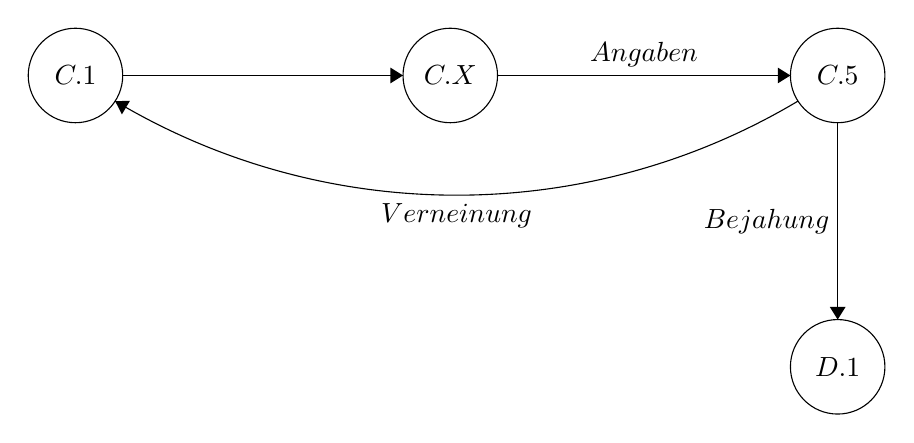
\begin{tikzpicture}[scale=0.2]
\tikzstyle{every node}+=[inner sep=0pt]
\draw [black] (5.4,-30.8) circle (3);
\draw (5.4,-30.8) node {$C.1$};
\draw [black] (29.2,-30.8) circle (3);
\draw (29.2,-30.8) node {$C.X$};
\draw [black] (53.8,-30.8) circle (3);
\draw (53.8,-30.8) node {$C.5$};
\draw [black] (53.8,-49.3) circle (3);
\draw (53.8,-49.3) node {$D.1$};
\draw [black] (8.4,-30.8) -- (26.2,-30.8);
\fill [black] (26.2,-30.8) -- (25.4,-30.3) -- (25.4,-31.3);
\draw [black] (32.2,-30.8) -- (50.8,-30.8);
\fill [black] (50.8,-30.8) -- (50,-30.3) -- (50,-31.3);
\draw (41.5,-30.3) node [above] {$Angaben$};
\draw [black] (53.8,-33.8) -- (53.8,-46.3);
\fill [black] (53.8,-46.3) -- (54.3,-45.5) -- (53.3,-45.5);
\draw (53.3,-40.05) node [left] {$Bejahung$};
\draw [black] (51.28,-32.427) arc (-59.18008:-120.81992:42.316);
\fill [black] (7.92,-32.43) -- (8.35,-33.27) -- (8.86,-32.41);
\draw (29.6,-38.9) node [below] {$Verneinung$};
\end{tikzpicture}
\end{center}

Folgendes gilt: 

\begin{enumerate}
\item{D.1 ist WELCOME}
\item{D.2 ist SEARCHCREATE}
\item{D.3 ist SEARCHPRODUCT}
\item{D.4 ist PRODUCTNAME}
\item{D.5 ist PRODUCTDESCR}
\item{D.6 ist PRODUCTPRICE}
\item{D.7 ist RESPONSE}
\item{D.X ist SEARCHAGAIN}
\item{X.S ist ENDE.SETNULLREP}
\item{X.A ist ENDE.ASKIFHAPPY}
\end{enumerate}

Basierend auf den ermittelten Nutzerinformationen wird nun eine Query erstellt. Dabei wird für jeden Nutzer eine Tabelle erstellt, die eine Kopie der originalen Datenbank ist. Diese wird im Schritt searchcreate erstellt. Daraufhin wird der Schritt SEARCHPRODUCT betreten, in der alle Artikel, die der Beschreibung des Nutzers entsprechen. In den den folgenden drei Regeln 'PRODUCTNAME', 'PRODUCTDESCR' und 'PRODUCTPRICE' jeweils Einträge aus Name, Beschreibung und Preis der Datenbank vorgestellt. In Response wird gefragt, ob dies dem Nutzerwunsch entspricht. Ist dies nicht der Fall, so wird in 'SEARCHAGAIN' übergegangen und erneut gesucht, wobei das bereits gefundene Produkt mit Hilfe der Eigenschaft 'queried' in der Datenbank (siehe \ref{sec:queried}) nicht erneut gefunden werden kann. Ist der Nutzer hingegen zufrieden, so wird dieser gefragt, ob dieser noch ein Produkt suchen will, ob dieser bereits Gewähltes einsehen will oder ob dieser fertig ist. Ist ersteres der Fall, so wird in die Regel 'SETNULLANDREP' im Topic 'Ende' weitergeleitet, sodass eine erneute Suche möglich ist. Ist zweiteres der Fall, so wird in der Datenbank erneut anhand der 'queried'-Eigenschaft eine Anfrage für alle Produkte aufgerufen, die akzeptiert worden sind. Will der Nutzer kein weiteres Produkt mehr suchen, so wird die Regel 'ASKIFHAPPY' in 'Ende' betreten.  
\begin{center}
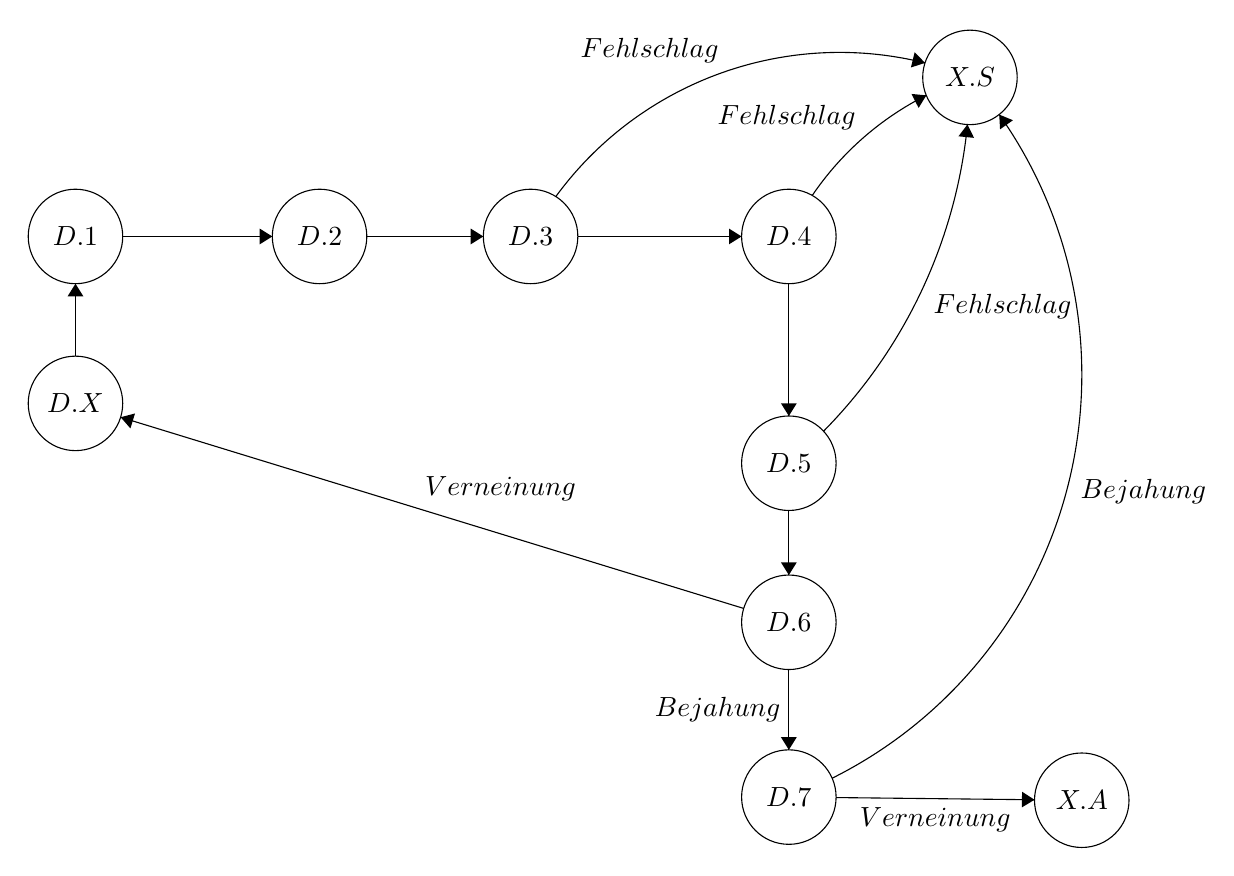
\begin{tikzpicture}[scale=0.2]
\tikzstyle{every node}+=[inner sep=0pt]
\draw [black] (8.1,-14.5) circle (3);
\draw (8.1,-14.5) node {$D.1$};
\draw [black] (23.6,-14.5) circle (3);
\draw (23.6,-14.5) node {$D.2$};
\draw [black] (37,-14.5) circle (3);
\draw (37,-14.5) node {$D.3$};
\draw [black] (64.9,-4.4) circle (3);
\draw (64.9,-4.4) node {$X.S$};
\draw [black] (53.4,-14.5) circle (3);
\draw (53.4,-14.5) node {$D.4$};
\draw [black] (53.4,-28.9) circle (3);
\draw (53.4,-28.9) node {$D.5$};
\draw [black] (8.1,-25.1) circle (3);
\draw (8.1,-25.1) node {$D.X$};
\draw [black] (53.4,-39) circle (3);
\draw (53.4,-39) node {$D.6$};
\draw [black] (53.4,-50.1) circle (3);
\draw (53.4,-50.1) node {$D.7$};
\draw [black] (72,-50.3) circle (3);
\draw (72,-50.3) node {$X.A$};
\draw [black] (11.1,-14.5) -- (20.6,-14.5);
\fill [black] (20.6,-14.5) -- (19.8,-14) -- (19.8,-15);
\draw [black] (26.6,-14.5) -- (34,-14.5);
\fill [black] (34,-14.5) -- (33.2,-14) -- (33.2,-15);
\draw [black] (38.603,-11.967) arc (143.8353:75.96593:22.332);
\fill [black] (62.05,-3.48) -- (61.39,-2.8) -- (61.15,-3.77);
\draw (44.56,-3.51) node [above] {$Fehlschlag$};
\draw [black] (54.885,-11.897) arc (145.81813:116.76502:19.213);
\fill [black] (62.13,-5.54) -- (61.19,-5.45) -- (61.64,-6.34);
\draw (53.26,-7.77) node [above] {$Fehlschlag$};
\draw [black] (53.4,-17.5) -- (53.4,-25.9);
\fill [black] (53.4,-25.9) -- (53.9,-25.1) -- (52.9,-25.1);
\draw [black] (40,-14.5) -- (50.4,-14.5);
\fill [black] (50.4,-14.5) -- (49.6,-14) -- (49.6,-15);
\draw [black] (64.743,-7.395) arc (-5.65741:-44.63217:32.239);
\fill [black] (64.74,-7.39) -- (64.17,-8.14) -- (65.16,-8.24);
\draw (62.56,-18.96) node [right] {$Fehlschlag$};
\draw [black] (8.1,-22.1) -- (8.1,-17.5);
\fill [black] (8.1,-17.5) -- (7.6,-18.3) -- (8.6,-18.3);
\draw [black] (53.4,-31.9) -- (53.4,-36);
\fill [black] (53.4,-36) -- (53.9,-35.2) -- (52.9,-35.2);
\draw [black] (53.4,-42) -- (53.4,-47.1);
\fill [black] (53.4,-47.1) -- (53.9,-46.3) -- (52.9,-46.3);
\draw (52.9,-44.55) node [left] {$Bejahung$};
\draw [black] (50.53,-38.12) -- (10.97,-25.98);
\fill [black] (10.97,-25.98) -- (11.59,-26.69) -- (11.88,-25.74);
\draw (35.09,-31.31) node [above] {$Verneinung$};
\draw [black] (66.756,-6.755) arc (35.24029:-63.48971:28.636);
\fill [black] (66.76,-6.76) -- (66.81,-7.7) -- (67.63,-7.12);
\draw (71.9,-30.73) node [right] {$Bejahung$};
\draw [black] (56.4,-50.13) -- (69,-50.27);
\fill [black] (69,-50.27) -- (68.21,-49.76) -- (68.19,-50.76);
\draw (62.69,-50.75) node [below] {$Verneinung$};
\end{tikzpicture}
\end{center}

Folgendes gilt:

\begin{enumerate}
\item{X.A ist askifhappy}
\item{X.B ist STILLHELP}
\item{X.C ist das Ablehnen einer weiteren Suche}
\item{X.D ist fgt}
\item{X.E ist goodbye}
\item{X.S ist SETNULLREP}
\item{firstq ist firstq aus Kaufabsicht}
\item{Z ist ein anderer Endzustand }
\end{enumerate}

Wird die Regel 'ASKIFHAPPY' in ENDE betreten, so wird dem Nutzer die Frage gestellt, ob man noch was für den Kunden tun könne, oder nicht. Ist dies nicht der Fall, so wird im folgenden die Datenbank für den Nutzer gedroppt und der Bot Beendet (X.E). Ist dies jedoch der Fall, so wird in 'STILLHELP' gefragt, ob man eine neue Suche starten wolle. Ist dies nicht der Fall, so wird der Bot beendet. Andererseits wird in 'SETNULLUNDREP' übergegangen, wo für die Kaufberatung relevanten Variablen zurückgesetzt werden und anschließend 'FIRSTQ' im Topic 'Kaufabsicht' betreten, zur erneuten Suche eines Produkts. 

\begin{center}
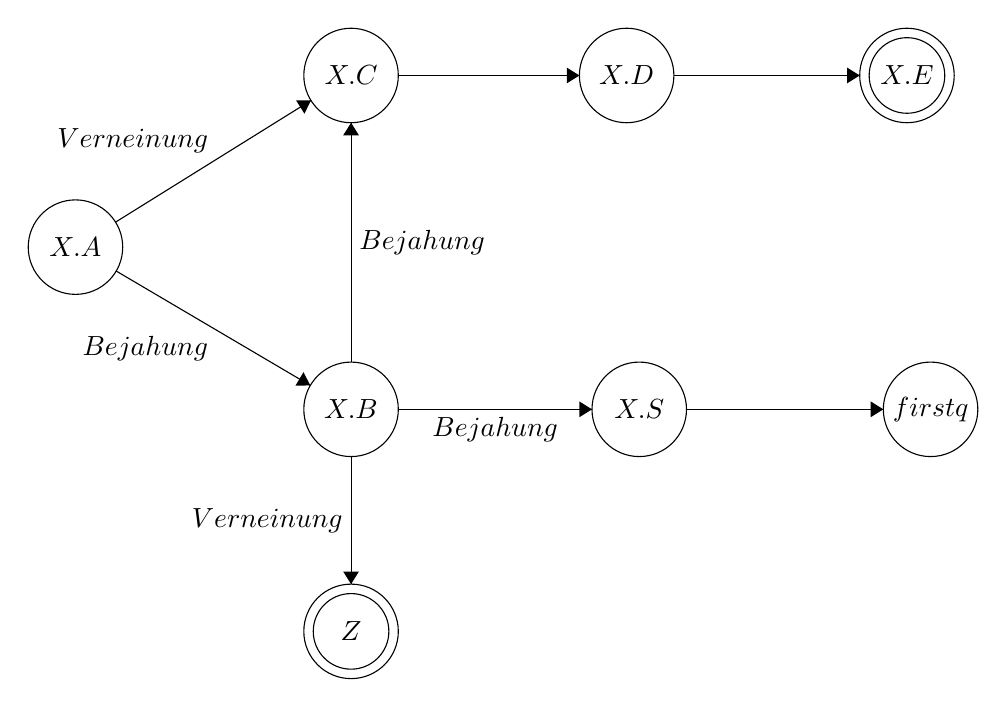
\begin{tikzpicture}[scale=0.2]
\tikzstyle{every node}+=[inner sep=0pt]
\draw [black] (6.7,-28.2) circle (3);
\draw (6.7,-28.2) node {$X.A$};
\draw [black] (24.2,-38.5) circle (3);
\draw (24.2,-38.5) node {$X.B$};
\draw [black] (24.2,-17.3) circle (3);
\draw (24.2,-17.3) node {$X.C$};
\draw [black] (24.2,-52.6) circle (3);
\draw (24.2,-52.6) node {$Z$};
\draw [black] (24.2,-52.6) circle (2.4);
\draw [black] (41.7,-17.3) circle (3);
\draw (41.7,-17.3) node {$X.D$};
\draw [black] (59.5,-17.3) circle (3);
\draw (59.5,-17.3) node {$X.E$};
\draw [black] (59.5,-17.3) circle (2.4);
\draw [black] (42.5,-38.5) circle (3);
\draw (42.5,-38.5) node {$X.S$};
\draw [black] (61,-38.5) circle (3);
\draw (61,-38.5) node {$firstq$};
\draw [black] (9.29,-29.72) -- (21.61,-36.98);
\fill [black] (21.61,-36.98) -- (21.18,-36.14) -- (20.67,-37);
\draw (11.13,-33.85) node [below] {$Bejahung$};
\draw [black] (9.25,-26.61) -- (21.65,-18.89);
\fill [black] (21.65,-18.89) -- (20.71,-18.88) -- (21.24,-19.73);
\draw (10.34,-22.25) node [above] {$Verneinung$};
\draw [black] (24.2,-35.5) -- (24.2,-20.3);
\fill [black] (24.2,-20.3) -- (23.7,-21.1) -- (24.7,-21.1);
\draw (24.7,-27.9) node [right] {$Bejahung$};
\draw [black] (24.2,-41.5) -- (24.2,-49.6);
\fill [black] (24.2,-49.6) -- (24.7,-48.8) -- (23.7,-48.8);
\draw (23.7,-45.55) node [left] {$Verneinung$};
\draw [black] (27.2,-17.3) -- (38.7,-17.3);
\fill [black] (38.7,-17.3) -- (37.9,-16.8) -- (37.9,-17.8);
\draw [black] (44.7,-17.3) -- (56.5,-17.3);
\fill [black] (56.5,-17.3) -- (55.7,-16.8) -- (55.7,-17.8);
\draw [black] (27.2,-38.5) -- (39.5,-38.5);
\fill [black] (39.5,-38.5) -- (38.7,-38) -- (38.7,-39);
\draw (33.35,-39) node [below] {$Bejahung$};
\draw [black] (45.5,-38.5) -- (58,-38.5);
\fill [black] (58,-38.5) -- (57.2,-38) -- (57.2,-39);
\end{tikzpicture}
\end{center}